\section{DATA PREPARATION AND HANDLING}

The data for this paper were organized with possible scalability in mind. The source of the dataset is the Operational Data Integrator (ODIN) PostgreSQL database maintained by Brazilian Airspace Control Institute (ICEA); the records collected range from January 1 to December 31, 2025. Extraction was performed using Python scripts that produced Parquet files optimized for analytical workloads and stored locally. Subsequent data transformation employed DuckDB as the query engine, with transformations orchestrated through data build tool (dbt), forming a Medallion Architecture data pipeline \cite{databricks_medallion, saha_dataeng}. The resulting datasets were again exported as Parquet files for downstream analysis in Python. The stack used for this work is schematized on Figure \ref{fig:odin-etl-simplified}.

\begin{figure}[htbp]
    \centering
    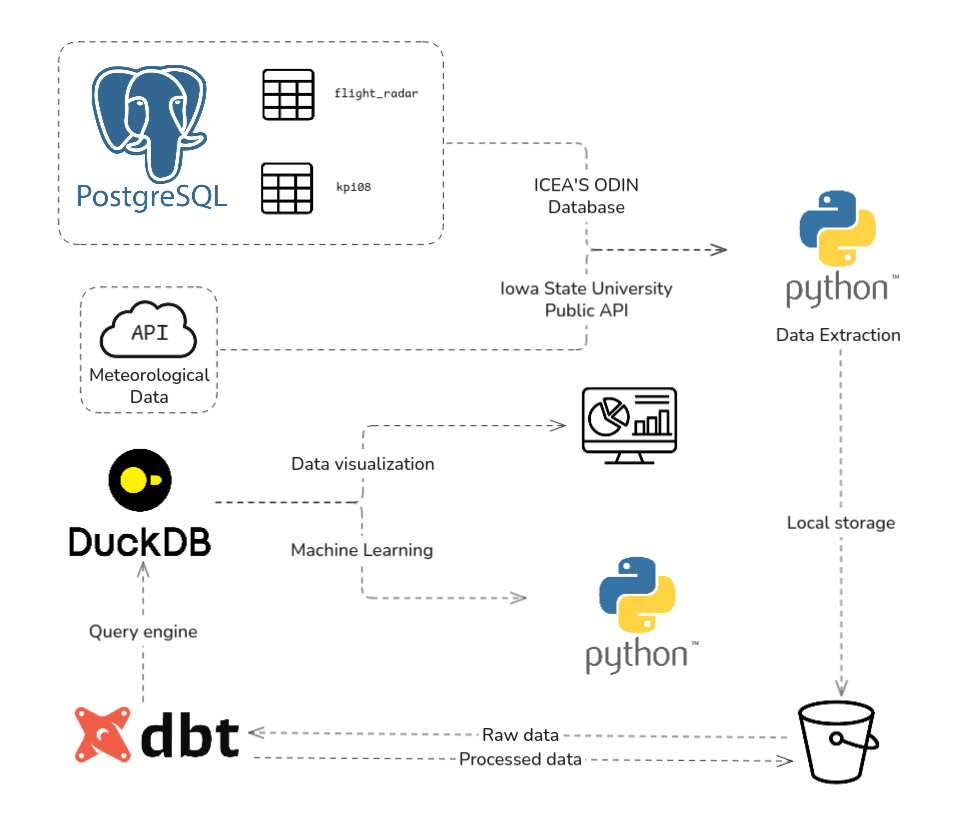
\includegraphics[width=1\linewidth]{images/odin-etl-simplified.png}
    \caption{Simplified schematics for the stack used in this work.}
    \label{fig:odin-etl-simplified}
\end{figure}

\subsection{FEATURE ENGINEERING}

To enhance the analytical value of the flight data, a series of feature engineering transformations were applied using DuckDB and subsequently orchestrated and documented through dbt. We focused on creating features that better represented flight behavior, airspace congestion, and operational context.

The data transformations were structured across multiple SQL models to progressively build the final dataset:

\begin{itemize}
    \item \textbf{Trajectory Tracking and Elapsed Time:} The radar trajectory points were bounded between the time the aircraft crossed the TMA cylinder (\textit{c\_time}) and the actual landing time (\textit{aldt}). For each flight level (FL) recorded, the time difference between consecutive radar pings was calculated to establish the \textit{elapsed} time spent at each altitude.
    
    \item \textbf{Fuel Consumption Estimation:} The \textit{elapsed} time per flight level was multiplied by the aircraft's specific average fuel flow rate (kg/s) obtained from the BADA performance tables \cite{bada_a320, pybada}. The sum of these values across all flight levels yielded the total fuel consumption in the terminal area (\textit{consumption\_kg}).
    
    \item \textbf{Airspace Congestion Tracking:} To represent the dynamic traffic density, an event-based running sum was implemented. Every \textit{c\_time} was treated as an entry (+1) and every \textit{aldt} as an exit (-1). Using SQL window functions over the chronological timeline, we calculated the exact number of aircraft present in the TMA at any given moment (\textit{nr\_aircraft\_in\_tma}).
    
    \item \textbf{Rolling Predictive Metrics:} A moving average for the time spent in the TMA (\textit{transit\_tma\_predicted}) was created to mimic the expected transit time given recent conditions. This was calculated over a 1-hour rolling window preceding the flight, partitioned by the validated runway (\textit{drwy\_validado}) and the entry sector (\textit{setor}).
    
    \item \textbf{Baseline Efficiency and Target Variable:} To define a standard for efficient operations, we calculated the 20th percentile of fuel consumption (\textit{consumption\_20p}) partitioned by departure airport (\textit{adep}), aircraft type, and landing runway. Finally, the main target variable for this study, \textit{kpi16}, was computed as the difference between the actual fuel consumption (\textit{consumption\_kg}) and this 20th percentile baseline.
    
    \item \textbf{Temporal and Environmental Variables:} Datetime fields were decomposed into specific categories (\textit{day}, \textit{month}, \textit{hour}, and \textit{day of week}) to capture seasonal and daily patterns. Additionally, weather information from the METAR database (Iowa State University public API) was joined by the hour, incorporating horizontal visibility and cloud ceiling to assess their impact on flight holding and routing.
\end{itemize}

These transformations—ranging from chronological event tracking to percentile-based baselining—were carefully designed to expose underlying trends, airspace bottlenecks, and correlations within the flight data, paving the way for sophisticated machine learning investigations. Furthermore, adopting structured data modeling approaches (e.g., Medallion architecture) ensures scalability when applying these pipelines to massive Apache Spark or distributed SQL environments \cite{databricks_medallion, saha_dataeng}.